\documentclass[tikz,border=3pt]{standalone}
\usetikzlibrary{arrows.meta}
\usepackage{amsmath,bm}
\let\boldsymbol\bm
\begin{document}
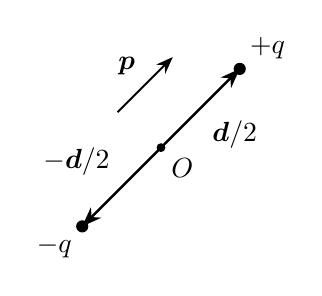
\begin{tikzpicture}[scale=1.0,>=Stealth,line width=0.9pt]
  \coordinate (O) at (0,0);
  \coordinate (P) at (1.0,1.0);
  \coordinate (M) at (-1.0,-1.0);

  % 原点 O から +q, -q へのベクトル d/2, -d/2
  \draw[->] (O) -- (P);
  \draw[->] (O) -- (M);

  % 原点・電荷の点
  \fill (O) circle (1.6pt) node[below right] {$O$};
  \fill (P) circle (2.2pt) node[above right] {$+q$};
  \fill (M) circle (2.2pt) node[below left] {$-q$};

  % ベクトルラベル
  \node[below right] at (0.52,0.48) {$\boldsymbol{d}/2$};
  \node[above left] at (-0.52,-0.48) {$-\boldsymbol{d}/2$};

  % 双極子モーメント p の向き
  \draw[line width=0.7pt,->] (-0.55,0.45) -- (0.15,1.15) node[midway,above left] {$\boldsymbol{p}$};
\end{tikzpicture}
\end{document}
